%% Index properties
%
% What a type says about its indices, read back by the layouts: where its
% index down the site leaves -- T's from its corner, and the stack moves T
% across so that the corner is on the site's line (tn leg anchor); which way
% it points, which the arrow on its bond follows (tn points); and the
% side on which it has one index however many sites it spans -- S, below
% (tn single). The triangles have them built in; any outline can be given them.
\documentclass[border=4pt]{standalone}
\usepackage{tikz-tensors}
\begin{document}
\begin{tikzpicture}
  \tnstack{S}{2}{a, b}
  \tnlayer{S}{a}{{tn box, tn leg anchor=south west}/$T$, {tn box, tn points=left}/$P$}
  \tnlayer{S}{b}{2*tn box/$A$}
  \tnconnect[along=tn arrow]{S}
  \tnstack{R}{2}{a}
  \tnlayer{R}{a}{{tn rounded, tn single=down}/$S$/2}
  \tnopen{up}{R}
  \tnopen{down}{R}
\end{tikzpicture}
\end{document}
